\documentclass{whutmod}
\usepackage{metalogo}
\usepackage{enumitem}
\usepackage{graphicx}
\usepackage{subfigure}
\usepackage {mathtools}
\usepackage{algorithm}  
\usepackage{algorithmicx}  
\usepackage{algpseudocode}  
\usepackage{float}
\usepackage{listings}
\usepackage{color}
\usepackage{amsmath}%添加矩阵宏包
\graphicspath{{figures/}} %图片在当前目录下的figures还有目录picture下,还可以继续添加其他搜索路径
\definecolor{dkgreen}{rgb}{0,0.6,0}
\definecolor{gray}{rgb}{0.5,0.5,0.5}
\definecolor{mauve}{rgb}{0.58,0,0.82}
\definecolor{backcolour}{rgb}{0.95,0.95,0.95}
\lstset{frame=tb,
	language=Python,
	backgroundcolor=\color{backcolour},   
	aboveskip=3mm,
	belowskip=3mm,
	showstringspaces=false,
	columns=flexible,
	basicstyle={\small\ttfamily},
	numbers=none,
	numberstyle=\tiny\color{gray},
	keywordstyle=\color{blue},
	commentstyle=\color{dkgreen},
	stringstyle=\color{mauve},
	breaklines=true,
	breakatwhitespace=true,
	tabsize=3
}
%插入参考文献命令
\newcommand{\upcite}[1]{\textsuperscript{\textsuperscript{\cite{#1}}}}

\renewcommand{\algorithmicrequire}{\textbf{Input:}}  % Use Input in the format of Algorithm  
\renewcommand{\algorithmicensure}{\textbf{Output:}} % Use Output in the format of Algorithm  
\team{26}	% 组号
\membera{许鸢飞}
\joba{编程}
\memberb{尹可汗}
\jobb{编程}
\memberc{李想}
\jobc{建模}
\title{基于数据上采样和贝叶斯优化的xgboost集成决策树红酒质量预测模型}
\tihao{5} % 题号

\begin{document}

\maketitle
%摘要
\begin{abstract}
	本文根据红酒的理化性质和数据特征,建立了基于数据上采样技术和贝叶斯优化的xgboost集成决策树红酒质量预测模型,实现了对红酒数据集质量的合理预测。
	~\\
	
	针对问题一,本文建立了以\textbf{决策树分类原理}为基础的\textbf{xgboost多分类器红酒预测模型}。首先,本模型对数据集进行了预处理工作,对于\textbf{数据缺失}的部分数据,我们采用均值进行填充,然后利用数据\textbf{归一化}消除了量纲之间的差异,并画出了各项指标的\textbf{分布特征},然后将处理完成的数据集,通过xgboost构建多分类器系统,利用\textbf{集成学习和梯度提升}的思想,通过\textbf{最佳分割点搜索算法},最终得到预测效果最好的多分类器系统。\textbf{该模型通过交叉验证在训练集上的预测率为62.8\%}。
	~\\
	
	针对问题二,\textbf{本文建立了基于皮尔逊相关性和xgboost叶节点权重的红酒重要指标提取和质量评估模型。}首先本文对问题一中的模型结构和属性进行提取,从而得到该模型在xgboost重要性计算中的多组排序方式,并利用归一化后的指标对其进行\textbf{皮尔逊相关性检验},从而得到各个指标之间还有质量之间的相关度,并结合参考文献得到重要程度较高的前3个量为\textbf{密度,酒精,剩余糖分,所占的影响比例分别为11.04\%,10.59\%,9.72\%,}同时对待测数据集进行了利用建立的模型进行了预测,并通过\textbf{灵敏度分析}可以得到\textbf{在合适的范围内,酒精浓度的增大,红酒质量能得到提升,剩余糖分过多会影响品质。}
	~\\
	
	针对问题三,本文利用\textbf{数据上采样和贝叶斯优化器}对xgboost模型从数据处理和模型参数进行了优化。首先我们通过分析当前数据集中的数据分布状况,可以看出等级为3,4,8,9的数量只占到7.6\%,存在明显的\textbf{数据分布不均衡}问题,于是本文利用数据上采样的\textbf{SMOTE算法},对当前少数类的样本以\textbf{k近邻搜索和欧氏距离差异}评价的方式构造出相同类型的新数据来填充少数类样本从而使得样本分布均衡化,然后利用\textbf{贝叶斯优化器}方法,利用先验概率与后验概率的关系对模型的树结构进行调整。\textbf{在上述优化方法下该模型的准确率达到了68.4\%,比问题一提升了5.6\%,}并对各参数进行了\textbf{灵敏度分析},从而得出了各超参数对于模型准确性的影响。
	~\\
	
	本文的优点:1.本文利用集xgboost集成学习的方法,建立多决策树分类器系统,有效防止模型预测出现过拟合。2.采用数据上采样方法合理构造新数据以扩充数据集保证样本类别的均衡分布,提高预测精度。
	
	
	\keywords{
		数据上采样 \quad
		贝叶斯优化 \quad
		xgboost \quad
		集成学习 \quad
		
	}
\end{abstract}

\tableofcontents
\newpage

\section{问题重述}
\subsection{问题背景}
改革开放40年来,中国葡萄酒行业实现了跨越式发展,中国即将超越英国成为仅次于美国的全球葡萄酒消费第二大市场。中国的年轻人已经将引用葡萄酒当做是一种社会时尚,葡萄酒正在征服年轻人的味蕾,并成为一种身份象征。

然而,市场上红酒的品质参差不齐,传统上葡萄酒的品质坚定大多依靠经验丰富的品酒师进行打分来判定,品酒师主要依据葡萄酒的外观,香气,口感和整体感觉等指标判断葡萄酒的品质.这种判定方式不仅会消耗大量人工成本和时间成本,而且品酒师的个人喜好也会对葡萄酒品质评价造成影响。在红酒种类越来越丰富的今天,这种评价方式显然难以满足市场的需求,葡萄酒品质评价工作迫切需要一种客观的,高效的鉴定方法.
图\ref{boerduo}是名声享誉海外的法国波尔多葡萄酒的分级图:
\begin{figure}[!htbp]
	\centering
	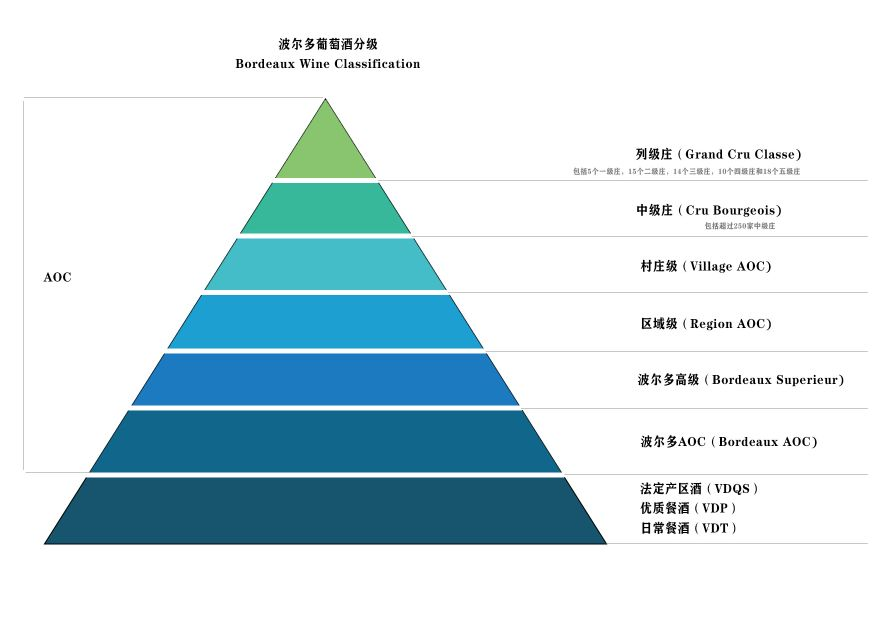
\includegraphics[width=0.8\textwidth]{boerduo3.jpg}
	\caption{波尔多葡萄酒分级示意图}
	\label{boerduo}
\end{figure} 


%\begin{figure}[!htbp]
%	\centering
%	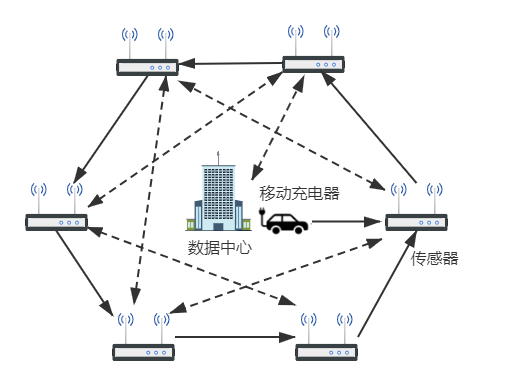
\includegraphics[width=0.6\textwidth]{系统示意图.png}
%	\caption{无线可充电网络示意图}
%	\label{示意图}
%\end{figure} 
\subsection{待解决的问题}
确定葡萄酒质量时一般是通过邀请一批有经验的品酒师对葡萄酒样品进行点评完成的。每个品酒师会对葡萄酒的外观,香气,口感和整体感觉四个方面进行评价,然后给出一个综合评分。这种评价方法的好处是有资质品酒师能凭借其专业水平区分葡萄酒间质量的差异,但缺点是这种评价方式效率低下,花费不菲且受到强烈的个人偏好的影响。葡萄酒质量评定需要一种基于算法的,客观的评价方法.附件一中给出了3898份葡萄酒样品的理化指标,题目要求我们根据这些特征建立分类模型,对红酒品质进行分类和预测,讨论以下问题:

1.对附件一中数据进行预处理,利用预处理后的数据建立合理的数学模型.

2.利用已建立的数学模型对待预测的红酒样品进行品质预测,并给出准确率分析,基于已建立的模型,运用新的模型找出影响红酒品质的前三中理化指标.

3.对建立的模型进行改进以提高分类的精确率,并展示优化效果.



\section{模型假设}
\begin{enumerate}
	\item 不考虑红酒样品非给定的11个理化指标对品质的影响,即红酒品质仅受题目所提供的理化指标数据的影响.
	\item xgboost模型的正确率和模型的超参数服从高斯过程,即具有特点的平滑性.据此在改进模型时我们根据贝叶斯优化方法对模型的超参数进行调优.
\end{enumerate}


\section{符号说明}
\begin{center}
	\begin{tabular}{ccccc}
		\toprule[1.5pt]
		符号 & 含义\\
		\midrule[1pt]
		$X_{ij}$ & 第j份红酒样品在第i项理化指标上的数据值\\
		$X'_{ij}$ &归一化处理后的数据\\
		$\overline X_{i}$ &第i项理化指标的平均值\\
		$\delta_{i}$ &第i项理化指标数据的标准差\\
		$P_{ij}$ &第$i$个样本在第$j$类理化指标上的预测概率\\
		$y_{ij}$ &第$i$个样本在第$j$类理化指标上的真实得分\\
		$T$ &叶子节点的个数\\
		$\omega_{j}$ &叶子节点在$j$类理化指标上的分数\\
		\bottomrule[1.5pt]
		注:表中未说明的符号以首次出现处为准
	\end{tabular}
\end{center}



\section{问题一模型的建立与求解}
\subsection{数据预处理}
数据集中共有3898个红酒样品的数据,包括11项红酒理化数据和一项评分数据,各项理化数据中有31个数据缺失,需要注意的是,理化数据的指标由于量纲不同,需要进行归一化处理。
\subsubsection{缺失值处理}
对于数据中存在对的确实现象,本文采用均值替换法对这种确实数据进行处理.

均值替换法就是将该项目剔除异常数据后取剩余数据的平均值来替换异常或缺失数据的方法:
\begin{equation}
\widetilde X_{ij}=\frac{1}{\hat n }\sum_{D}X_{i}.
\end{equation}
其中,$\widetilde X_{ij}$表示缺失值,$\hat n$表示完好数据的数量,$\sum_{D}X_{i}$表示第$i$项理化指标完好数据的加和.

\subsubsection{数据归一化处理}
不同理化指标的绝对值存在数量级上的差异,可能会影响模型建立的可靠性,我们对数据进行标准化处理,某个数据减去该项指标数据平均值再除以相应的标准差:

对于任意数据$X_{ij}$,$i$表示第$i$项理化指标,$j$表示第$j$份红酒样的该项指标上的数据值.$\overline X_{i}$表示第{i}项理化指标的平均值.$\delta_{i}$表示第$i$项理化指标的标准差,处理后的数据用$X'_{ij}$表示:
\begin{equation}
X'_{ij}=\frac{X_{ij}-\overline X_{i}}{\delta_{i}}.
\end{equation}

\subsubsection{数据分布}
利用题中所给数据我们进行了可视化处理,画出了3898种红酒样品理化指标和分级的直方图与归一化处理后数据的箱线图,由于图像过大,我们将其置于目录中.我们发现:
\begin{figure}[!htbp]
	\centering
	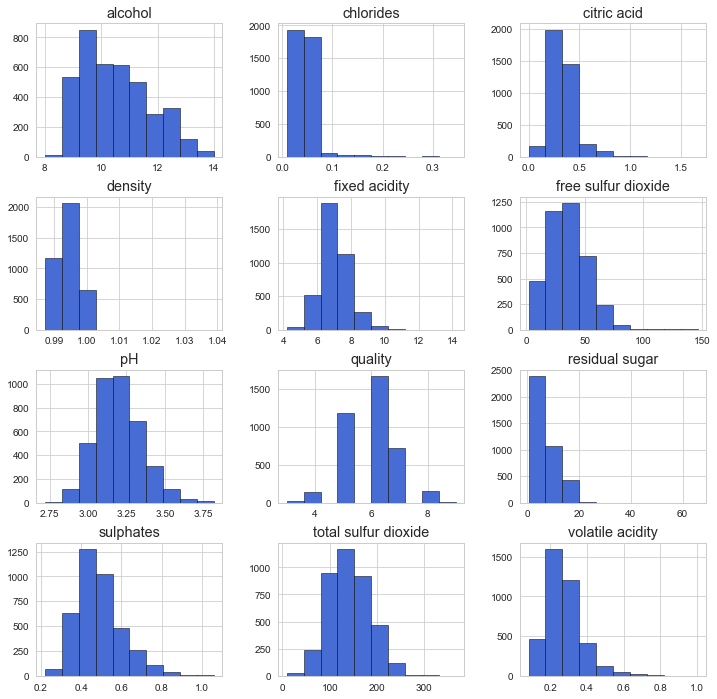
\includegraphics[width=0.6\textwidth]{fenbu.png}
	\caption{原始数据分布}
\end{figure} 

\textbf{1.}11项理化指标数据呈现明显的正偏态.即各项数据中众数<中位数<平均数.其中氯化物,挥发性酸和游离二氧化硫的右偏程度较大,而总二氧化硫,酸碱度和酒精度的右偏程度较小。

\textbf{2.}每项理化数据间的极差相差较大,总二氧化硫的极差为357.5,而密度间的极差仅为0.051,这说明了数据归一化的重要性.

\textbf{3.}我们发现红酒的质量评分集中在5,6,7等.品质分级在4等以下或8等以上的红酒较少.


\subsection{问题分析}
在问题一中,我们需要对题中给出的训练集进行缺失值,归一化等特征工程处理,然后对预处理以后的数据来建立合理的模型来对红酒数据集进行分类识别,对于分类算法来说比较传统的是决策树分类模型,朴素贝叶斯分类算法,而这些方法的实现往往评判比较单一,且决策树具有天然的过拟合问题,所以在小样本的情况下,容易出现过拟合问题,所以本文采用集成学习的思想,采用xgboost构建一个多决策树分类器系统来完成对该问题的分类,xgboost是一种高度可扩展的端到端的多学习器模型,能够更加高效的解决该问题,并有效防止过拟合。
%插入参考文献\upcite{bib:one}。
\begin{figure}[!htbp]
	\centering
	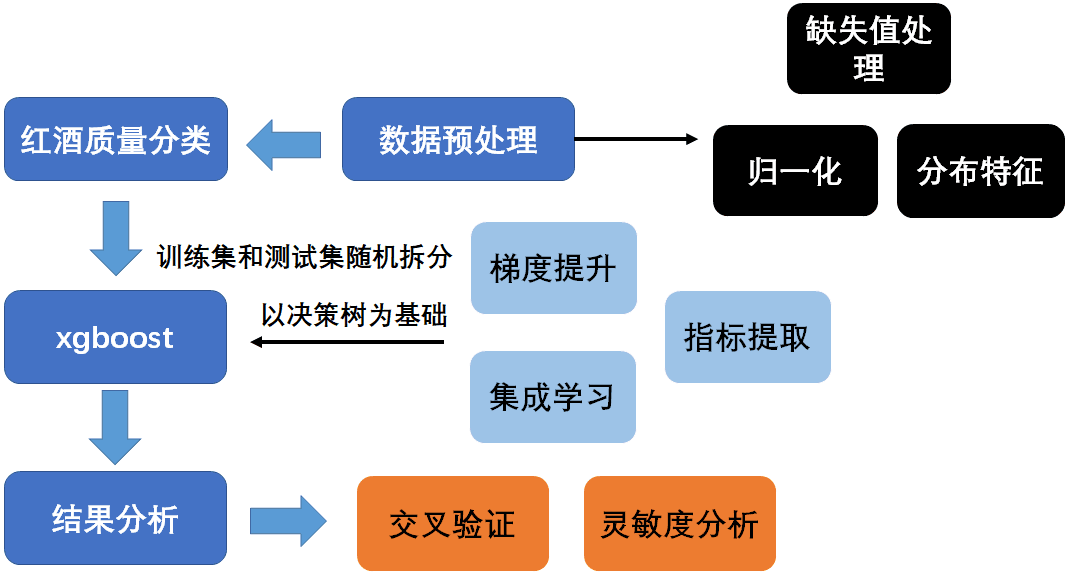
\includegraphics[width=0.7\textwidth]{map1.png}
	\caption{问题一思维导图}
\end{figure} 


\subsection{xgboost集成决策树红酒分类模型}

\subsubsection{梯度提升法多决策树系统构建}
xgboost构建多个分类器系统的思想是梯度提升的方式,最开始先建立一棵决策树树,然后逐渐迭代,每次迭代过程中都增加一棵树并通过调整使得他能减小当前的预测误差,逐渐形成众多树模型集成的强评估器。其中$f_k$表示第$k$棵决策树的计算函数, $x_i$表示样本$i$对应的特征向量,特征向量则是我们上述归一化后对应的理化指标$x_i=(X'_{i1},X'_{i2},...,X'_{in})$.

这里我们设$P_i={P_{i1},P_{i2},...,P_{in}}$表示第i棵决策树对当前样本预测得出的每一类的概率,令$P_{ij}$表示第$i$个样本在第$j$类上的预测概率,而概率最大的自然是被选择的样本预测结果,令$y_{ij}$表示第$i$个样本在第$j$类上的真实得分值,则我们可以构建一个葡萄酒等级的分类序列$\hat{y}_i=(y_{i1},y_{i2},y_{i3}...y_{in})$,那么我们就能得到xgboost中一棵决策树的样本预测结果和各类红酒等级的概率.
\begin{equation}
y_{ij}=\begin{cases} 
1,&\text{if $y_{ij}$=j}.\\
0,&\text{else}.
\end{cases}
\end{equation}
\begin{equation}
\hat{y}_i=\sum_{k=1}^Kf_k(x_i).
\end{equation}

\begin{figure}[!h]
	\centering
	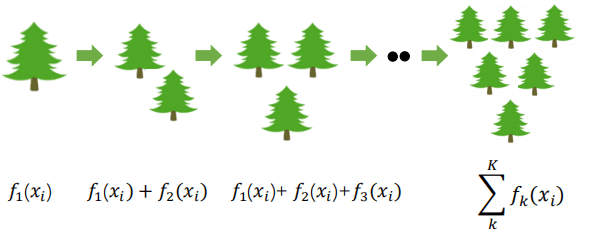
\includegraphics[width=0.8\textwidth]{tree.png}
	\caption{xgboost梯度提升树构建}
	
\end{figure}

\subsubsection{交叉熵损失函数}
为了缩小样本与预测值之间的差异,我们需要通过构建衡量样本与原始数据差异的损失函数,这里我们采用交叉熵的方式来计算两个样本之间的结果。
\begin{equation}
L=\frac{1}{n}\sum_{i=1}^NL_i=\frac{1}{N}\sum_{i=1}^NL_i-\sum_{j=1}^M
y_{ij}log(P_{ij}).
\end{equation}
其中$M$表示分类的样本数量,$P_{ij}$表示第$i$个样本在第$j$类上的预测概率,$y_{ij}$表示第$i$个样本在第$j$类上的真实得分,如果该类别和样本i的类别相同就是1,否则是0.$N$表示样本的个数。
\begin{equation}
\begin{aligned}
L(y, \hat{y}) &=\sum_{i=1}^{M} L\left(y_{i}, \hat{y}_{i}\right) \\
&=\sum_{i=1}^{M} L\left(\left(y_{i0}, y_{i1}, \ldots y_{iN-1}\right),\left(\hat{y}_{i0}, \hat{y}_{i1}, \ldots \hat{y}_{iN-1}\right)\right) \\
&=-\sum_{i=1}^{M} \sum_{n=0}^{N-1} y_{in} \log \left(\frac{e^{\hat{y}_{in}}}{\sum_{c=0}^{N-1} e^{\hat{y}_{ic}}}\right).
\end{aligned}
\end{equation}

\subsubsection{模型复杂度惩罚项}
同时为了保证该模型树的复杂度,我们在该损失函数中添加了惩罚项来限制树的模型,从而减小模型的叶子节点数目,树的深度,防止过拟合提高模型的泛化能力,也能减小运算的开销。
\begin{equation}
\Omega(f)=\gamma T+\frac{1}{2}\lambda ||w||^2=\gamma T+\frac{1}{2}\lambda \sum_{j=1}^T w_j^2.
\end{equation}
$T$表示叶子节点的个数,$w_j$表示叶子节点$j$上的分数。直观上看,目标要求预测误差尽量小,且叶子节点T尽量少($\gamma$ 控制叶子结点的个数),节点数值$w$尽量不极端($\lambda$控制叶子节点的分数不会过大),防止过拟合。

\subsubsection{优化目标函数}
为了在保证正确率和模型复杂度两者的情况下,我们通常在目标函数里需要将两者结合起来作为训练迭代的评判依据。
\begin{equation}
Obj=\sum_i^N L(y, \hat{y})+\sum_k^K \Omega(f_k).
\end{equation}
利用二阶泰勒展开法,可得到
\begin{equation}
Obj=\sum_{i=1}^N[f_k(x_i)g_i+\frac{1}{2}(f_k(x_i))^2h_i)]+\Omega(f_k).
\end{equation}
其中$g_i=\frac{\partial L(y, \hat{y}_{i}^{(t-1)})}{\partial \hat{y}_{in}^{(t-1)}},h_i=\frac{\partial^2 L(y, \hat{y}_{i}^{(t-1)})}{\partial \hat{y}_{in}^{(t-1)^2}}$
再通过整理操作得到
\begin{equation}
Obj=\sum_{j=1}^T[(\sum_{i \in I_j} g_i )w_j+\frac{1}{2}(\sum_{i \in I_j} h_i+\lambda)w_j^2]+\gamma T.
\end{equation}
$I_j$被定义成每个叶节点j上面样本下标的集合$I_j=\{i|f(x_i)=j\}$,为了简化公式则把求导部分记为$G_i=\sum_{i \in I_j} g_i$,$H_i=\sum_{i \in I_j} h_i$.
\subsection{模型求解}
当我们指定一个树的结构的时候,我们要对树的结构进行优化,我们将优化的程度称为结构分数.
\begin{equation}
Obj=-\frac{1}{2}\sum_{j}\frac{G_{j}^{2}}{H_{j}+\lambda}+7\gamma.
\end{equation}
\subsubsection{最佳分割点搜索算法}
为了确定树的结构,一个理所当然的想法就是不断枚举不同树的结构,然后利用打分函数来寻一个最优结构的树.本题提供了3989种红酒样品的数据,我们使用贪心法,从树深度为0开始,每一个节点都遍历所有的特征,如柠檬酸含量,酒精度等.对于某一特征,我们先按照该特征里的值进行排序,然后线性扫描该特征进而确定最好的分点,最后对所有特征进行分割后,我们选择增益$Gain$最高的那个特征.
\begin{equation}
Gain=\frac{1}{2}[\frac{G_{L}^{2}}{H_{L}+\lambda}+\frac{G_{R}^{2}}{H_{R}+\lambda}-\frac{(G_{L}+G_{R})^{2}}{H_{L}+H_{R}+\lambda}]-\gamma.
\end{equation}
其中$\frac{G_{L}^{2}}{H_{L}+\lambda}$表示左子树的分数,$\frac{G_{R}^{2}}{H_{R}+\lambda}$表示右子树的分数,$\frac{(G_{L}+G_{R})^{2}}{H_{L}+H_{R}+\lambda}$表示分割前的分数,$\gamma$表示加入新叶子节点引入的复杂度代价.

对于所有的特征,我们只用做一遍从左到右的扫描就可以枚举出所有分割的梯度和树左右的得分$G_{L}$和$G_{R}$.然后计算每个分割方案的得数就可以的.

值得注意的是引入分割不一定会使情况变得更好,所以我们有一个引入新叶子的惩罚项。优化这个目标对应了树的简枝,当引入的分割带来的增益小于一个阈值$\Upsilon$的时候,则忽略这个分割.
以下是优化树结构的贪心法的伪代码:
\begin{algorithm}
	\caption{Exact Greedy Algorithm for Split Finding}
	\begin{algorithmic}
		\Require I,当前节点的实例集
		\Require d,特征维度
		\State $gain \gets 0$  $G \gets \sum_{i\in I}g_{i},H \gets \sum_{i\in I}h_{i}$ 
		\For{$k = 1\quad to\quad m $}  
		\State $G_{L}\gets 0,H_{L} \gets 0$
		\For{$j\quad in\quad sorted(I,byx_{jk})$}
		\State $G_{L}\gets G_{L}+g_{j},H_{L} \gets H_{L}+h_{j}$ 
		\State $G_{R}\gets G-G_{L},H_{R} \gets H-H_{L}$ 
		\State $score\gets (score,\frac{G_{L}^{2}}{H_{L}+\lambda}+\frac{G_{R}^{2}}{H_{R}+\lambda}-\frac{G^{2}}{H+\lambda})\text{的最大值}$
		\EndFor
		\EndFor
		\Ensure 最高分数的优化
		
	\end{algorithmic} 
\end{algorithm}
\subsection{结果分析}
\subsubsection{xgboost分类结构}
通过训练和测试以后,我们利用python的xgboost.to\_graphviz函数将他对分类特征的处理进行详细的可视化,从而得到他的完整分类流程,该模型共生成了50多棵树,这里选取其中第一棵树的结构来做一个实例,来反映他的流程。
\begin{figure}[!h]
	\centering
	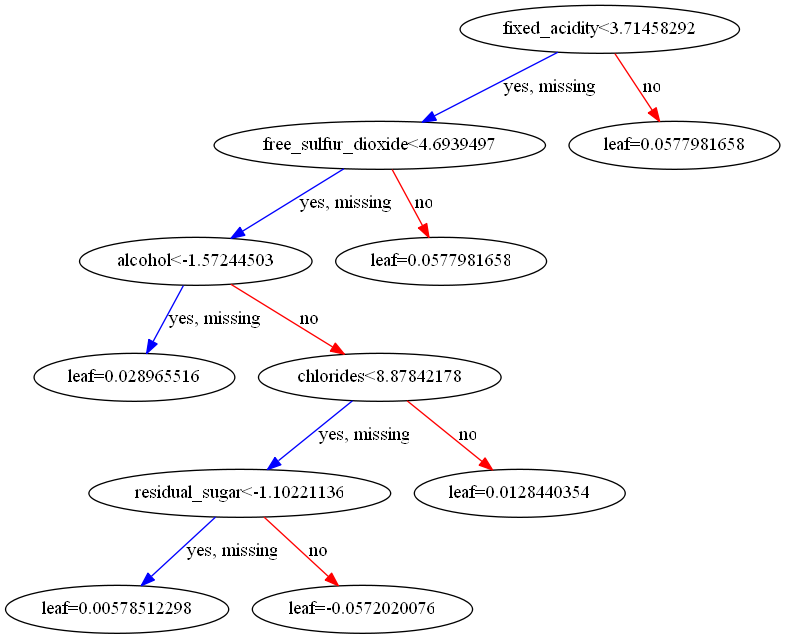
\includegraphics[width=0.6\textwidth]{xgbtree.png}
	\caption{xgboost中第一颗树的分类结构}
\end{figure}


\subsubsection{分类性能}
该模型通过交叉验证得到\textbf{该模型的正确率为}\textbf{62.8\%},当前查准率和查全率都为0.628说明,该模型的已经达到了识别分类的平衡点。

% Table generated by Excel2LaTeX from sheet 'Sheet1'
\begin{table}[!htbp]
	\centering
	\caption{模型泛化性能}
	\begin{tabular}{crrr}
		\toprule
		& \multicolumn{1}{c}{\textbf{微平均}} & \multicolumn{1}{c}{\textbf{宏平均}} & \multicolumn{1}{c}{\textbf{加权平均}} \\
		\midrule
		\textbf{查准率precision} & 0.628 & 0.496615 & 0.625077 \\
		\textbf{查全率recall} & 0.628 & 0.413332 & 0.628 \\
		\textbf{两者的调和平均F1-score} & 0.628 & 0.433917 & 0.617503 \\
		\bottomrule
	\end{tabular}%
	\label{tab:addlabel}%
\end{table}%
我们画出了红酒分类预测的等级混淆矩阵,如图\ref{cm1},矩阵对角线颜色较深,整体矩阵颜色较浅,说明预测偏差较少,且多发生相邻等级之间,证明了我们模型预测的可靠性.
\begin{figure}[!h]
	\centering
	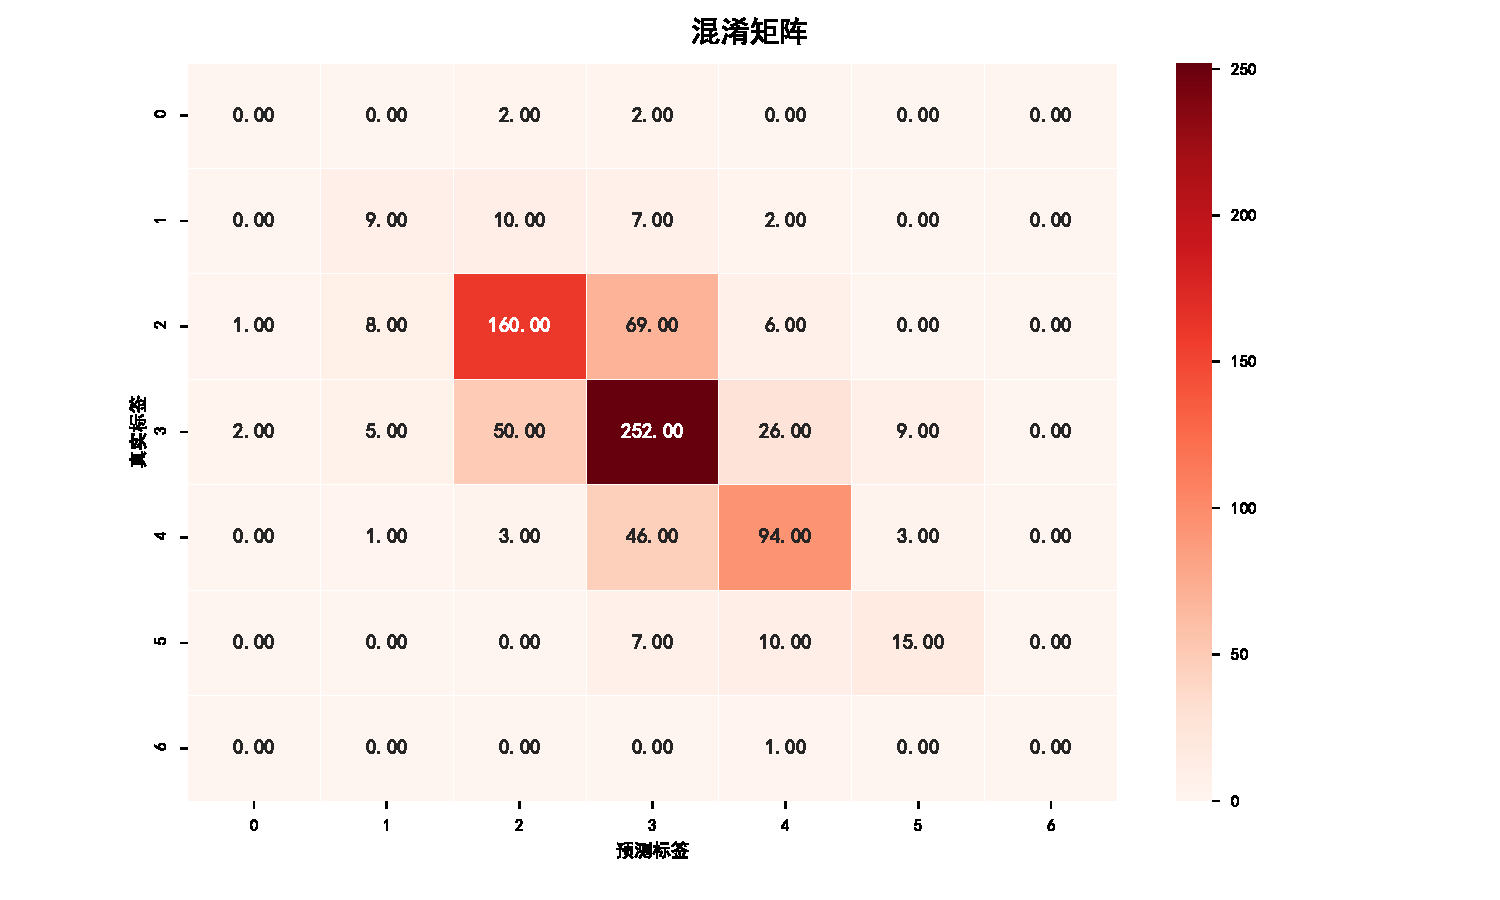
\includegraphics[width=0.8\textwidth]{cm1.pdf}
	\caption{红酒分类等级混淆矩阵}
\label{cm1}
\end{figure}
%\subsubsection{灵敏度分析}

\section{问题二模型的建立与求解}
\subsection{问题分析}
问题二要求我们使用问题一建立的模型对附件中的待预测数据集进行品质预测,同时运用合理的数学模型找出影响红酒品质的理化指标的前三名.我们使用的基于集成树思想的模型,利用了不同红酒样品在11种理化指标上的差距,对红酒品质完成了分类.对于模型一中使用的累加优化方法,一个特征出现时覆盖的样本数或者该特征带来的增益效果显然是影响红酒品质的重要指标.
\begin{figure}[!h]
	\centering
	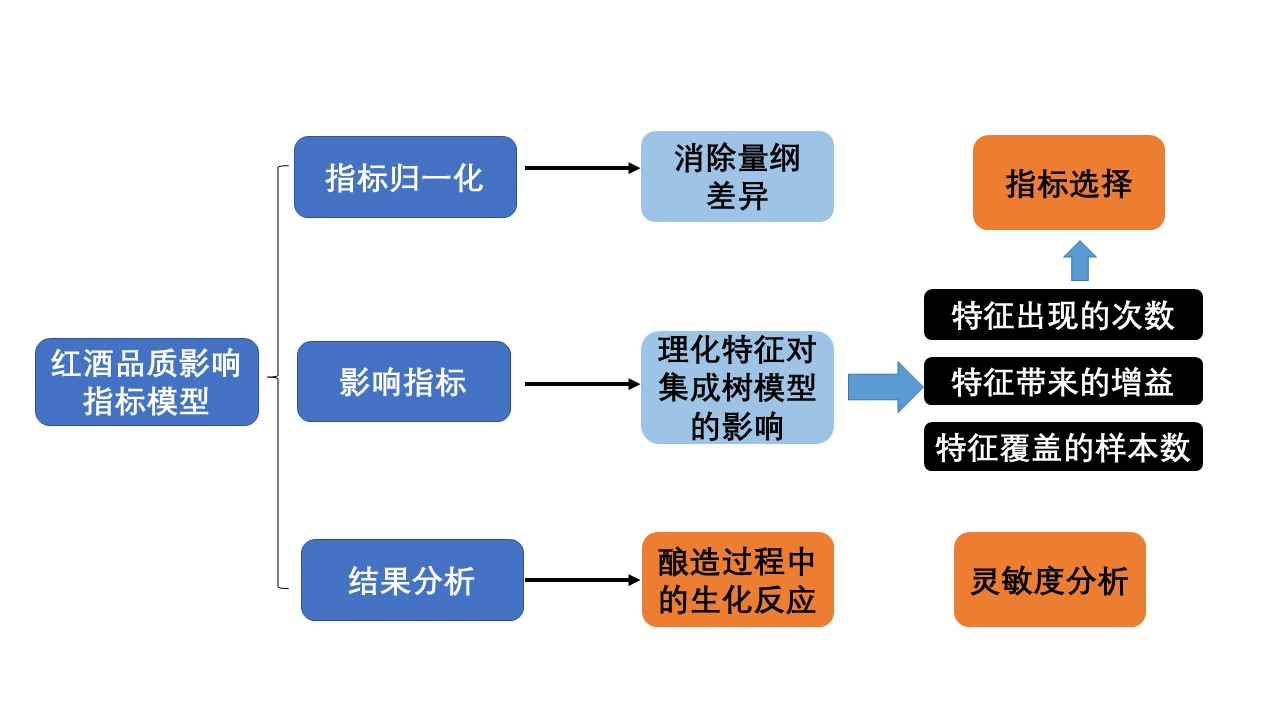
\includegraphics[width=0.7\textwidth]{map2.jpg}
	\caption{问题二思维导图}
\end{figure}
\subsection{红酒品质影响指标模型的建立}
我们认为一个特征在整个集成树模型中出现的次数越多,或者其特征作为树的分裂节点带来的增益总和越多,那么这项特征在对红酒进行分类时的影响就更大。

$xgboost$算法中有5种常见的计算特征重要性的指标;
\begin{itemize}
	\item{$weight$}:表示某种特征在整个树群节点中出现的次数,出现越多,价值就越高.
	
	\item{$gain$}:某特征在整个树群作为分裂节点的信心增益之和再除以某特征出现的频次,表示该特征出现带来的平均优化效果.
	
	\item{$cover$}:表示在树群中,一个特征作为分裂节点存在时,覆盖的样本数量的平均值.
	
	\item{$total gain$}表示某特征给树群带来的总增益的大小.
	
	\item{$tatal cover$}表示覆盖的样本总量.
\end{itemize}
我们的目的是找出影响红酒品质的前三的理化指标,并解释什么导致一种红酒的品质处于某一等级,所以我们选择的指标要能反映理化指标对红酒样品的平均影响,所以我们选择$gain$和$cover$和$weight$三个指标进行研究.
\begin{equation}
weight_{i}=N_{i},
\end{equation}
$N_{i}$表示第$i$种理化特征在整个树群节点中出现的次数
\begin{equation}
gain_{i}=\frac{\sum_{D}{Gain_{i}}}{n_{is}},
\end{equation}
其中,$n_{is}$表示第$i$种理化指标作为树分裂节点的次数.
\begin{equation}
cover_{i}=\frac{N_{i}}{n_{is}}.
\end{equation}
其中,$N_{i}$表示第$i$个理化指标作为分裂节点时,覆盖的样本总数.

\textbf{指标归一化}

我们已经得到了红酒不同理化指标上述两个指标上的得分情况,但这时的数据还只是得分的绝对表示,为了研究不同理化指标对红酒品质影响的排列顺序,我们需要将得分的绝对数转化为相对数,即百分比形式.

用$P_{wi}$表示第$i$种理化指标基于$weight$指标的得分情况.
\begin{equation}
P_{wi}=\frac{weight_{i}}{\sum_{D} weight{i}}\times 100\%,i=1,2,...11,
\end{equation}

用$P_{gi}$表示第$i$种理化指标基于$gain$指标的得分情况:
\begin{equation}
P_{gi}=\frac{gain_{i}}{\sum_{i=1}^{11}gain_{i}}\times 100\%,i=1,2...11,
\end{equation}

用$P_{ci}$表示第$i$种理化指标基于$cover$指标的得分情况:
\begin{equation}
P_{ci}=\frac{cover_{i}}{\sum_{i=1}^{11}cover_{i}}\times 100\%,i=1,2...11.
\end{equation}

\subsection{模型求解与分析}

\subsubsection{相关性分析}
我们画出了各个理化指标之间相关度的\textbf{热力图},如\ref{xiangguandu},可以看到:

\textbf{1.}红酒的质量评分与酒精、酸碱性、硫酸盐、游离二氧化硫有正的线性相关关系,它们的含量越高,口感评分越高;而与其他特征都呈现负的线性相关关系,这些特征的含量越高,口感评分越低.关系强度最大为0.45。

\textbf{2.}酒精度和密度之间的相关性为-0.77,两者存在较大相关性,且酒精度越高,密度越小。密度和残糖的相关性为0.84,两者的相关性较大,且残糖越高,密度越大.

\textbf{3.}从热力图上看,颜色普遍较浅,除极少对理化指标外,各理化指标之间的相关性较弱.

\begin{figure}[!h]
	\centering
	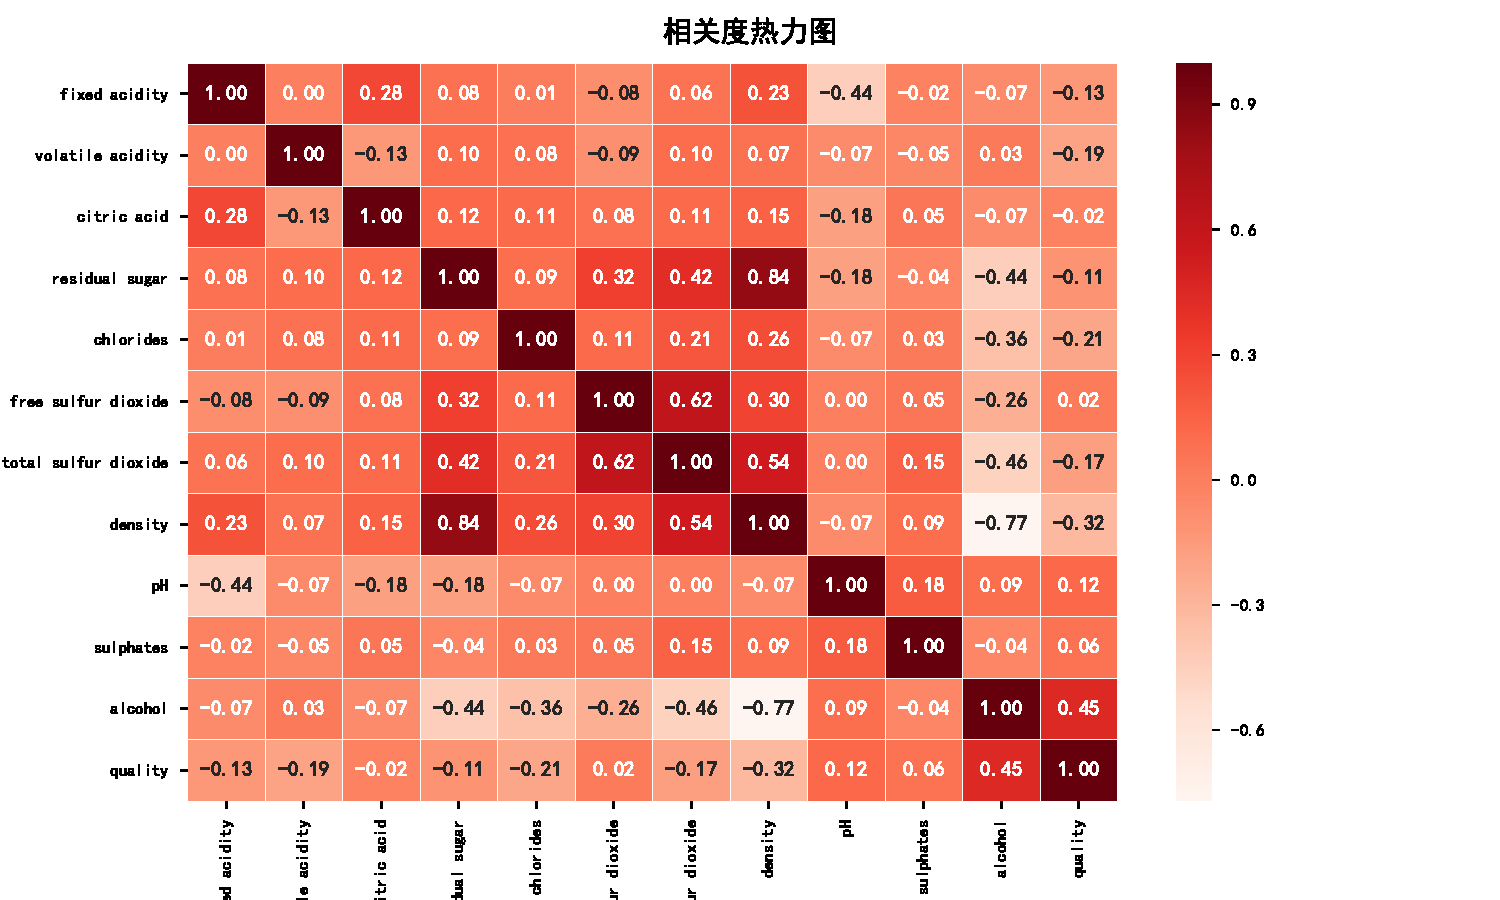
\includegraphics[width=0.8\textwidth]{_corr.pdf}
	\caption{各理化指标之间的相关度}
\label{xiangguandu}
\end{figure}

\subsubsection{指标选择}
我们使用$feature-importance$命令求出了各项理化数据在上述三个指标上的表现,在进行归一化后对各理化数据在三个指标上的影响分数进行累加,如图\ref{featureall}.
\begin{figure}[!h]
	\centering
	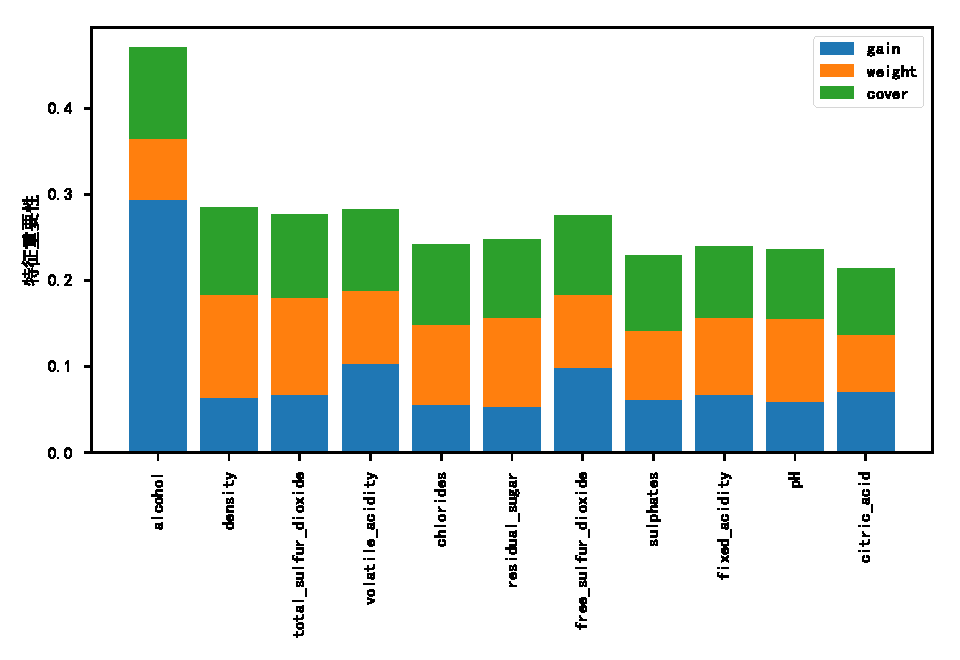
\includegraphics[width=0.8\textwidth]{featureall.pdf}
	\caption{各理化指标影响分数在三个指标上的累加}
\label{featureall}
\end{figure}

我们查阅了相关参考文献\upcite{bib:five},了解了葡萄酒理化指标对葡萄酒品质的影响,在综合各理化指标与质量的相关性和上述三个指标显示的影响得分后,我们最终选择了$cover$指标作为计算影响红酒品质的方法.图\ref{featurecover}展示了各理化指标在该标准下的影响分数:

\begin{figure}[!h]
	\centering
	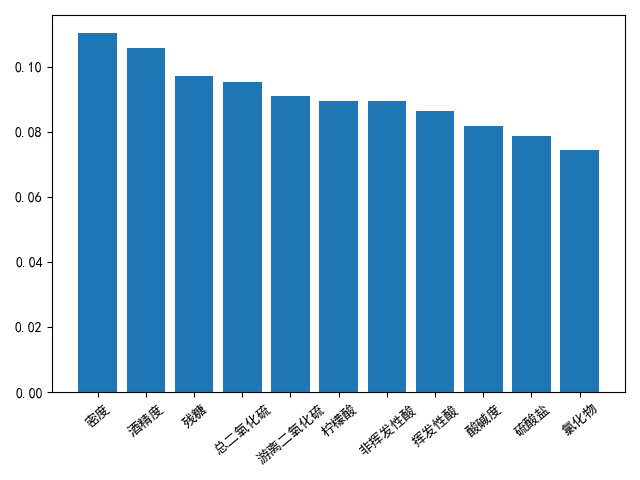
\includegraphics[width=0.8\textwidth]{res2.png}
	\caption{各理化指标影响分数在cover指标上的体现}
\label{featurecover}
\end{figure}

我们得到的影响红酒品质属性前三名的理化指标分别为\textbf{酒精度,密度和剩余糖分},影响分数分别为:\textbf{11.04\%,10.59\%,9.72\%}.

根据参考文献\upcite{bib:five}\upcite{bib:six},我们对上述三种理化指标对葡萄酒品质产生影响的机理做出解释:

\textbf{1.}酒精度是对葡萄酒品质影响最大的理化指标,在一定范围内,酒精度越高,说明葡萄酒发酵的时间越长,发酵选择的菌种越优良,在相关参考文献\upcite{bib:five}中选出的品质上乘葡萄酒中,酒精度都在$13.74\pm 0.67$度之间,这也解释了样本数据中80\%的品质为9级的红酒,酒精度都在12.4度以上.

\textbf{2.}不同红酒间密度的差异\upcite{bib:six} 主要是乙醇,糖类,各种酯类化合物,各种酸,色素造成的,这些经微生物发酵产生的化学物质,极大影响了红酒的颜色,口感,气味,是评价红酒品质的重要组成部分.

\textbf{3.}在红酒酿造过程中,核心生化反应是通过微生物将糖类转化为乙醇,同时,剩余的糖也会对红酒的口感造成影响,红酒中残存的糖过多,则说明酿造时间过短,糖份过少可能会导致红酒苦涩,残糖量是影响红酒口感的重要指标.

\subsubsection{待预测集品质预测}
根据问题一中建立的模型,对附件一种待预测集进行品质预测:
\begin{table}[!htbp]
	\caption{预测结果分布} \centering
	\begin{tabular}{cccccccccc}
		\toprule[1.5pt]
			等级 & 3 & 4 & 5 & 6 & 7 & 8 & 9 \\
		\midrule[1pt]
		数量 & 5 & 42 &355  & 260 & 267 &70  &1 \\
		\bottomrule[1.5pt]
	\end{tabular}
\end{table}

\begin{figure}[!h]
	\centering
	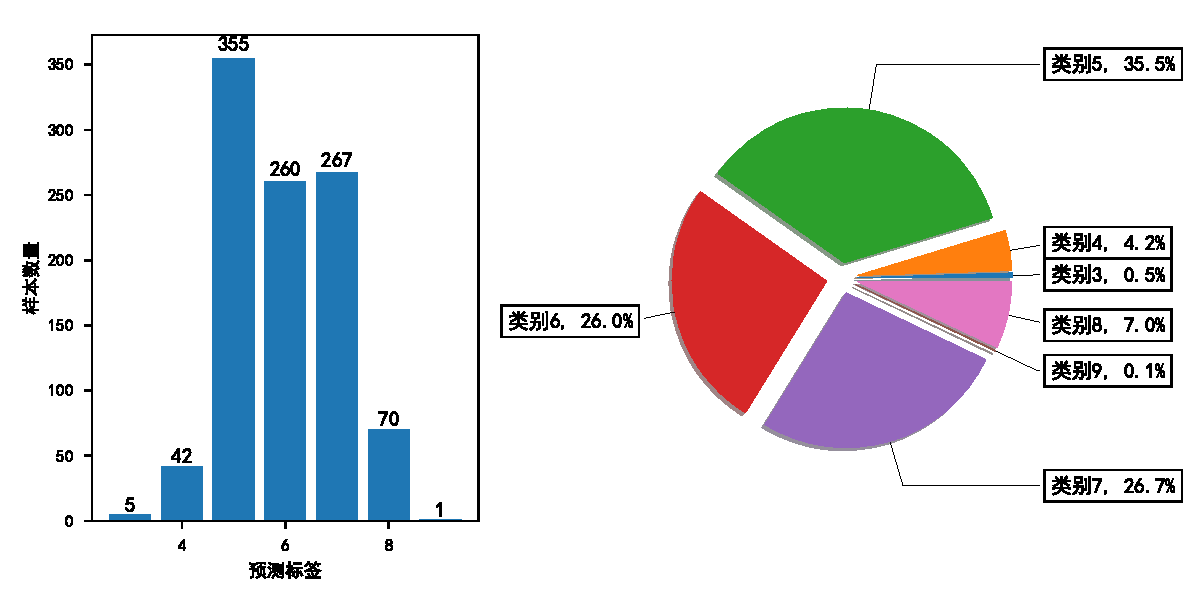
\includegraphics[width=0.8\textwidth]{labels_class_counts_test_pred.pdf}
	\caption{预测数据集质量分布}
\end{figure}

\subsection{灵敏度分析}
我们针对所选的重要指标对红酒品质的影响做灵敏度分析,通过随机选取10个样本,使其在参考文献所给的酒品正常规格内进行变化,并取这是个样本的均值可以看出.\textbf{在合适的范围内,酒精浓度的增大,红酒质量能得到提升,剩余糖分过多会影响品质。}
\begin{figure}[!h]
	\begin{minipage}[t]{0.48\textwidth}
		\centering
		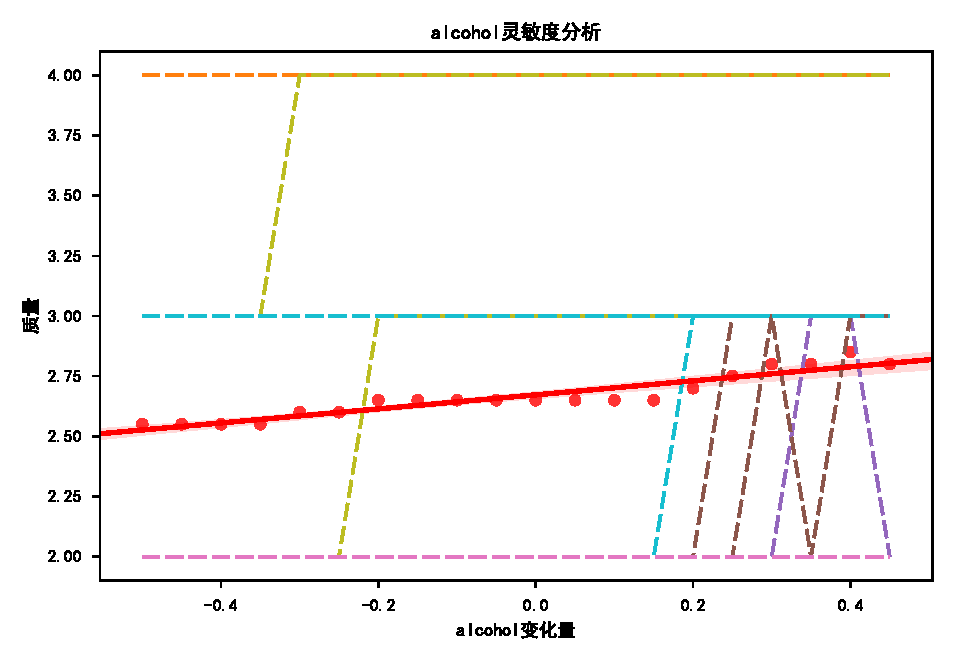
\includegraphics[width=0.99\textwidth]{sensitivity_alcohol.pdf}
		\caption{酒精含量变化对酒品质量的影响}
%		\label{fig:Anhui_loss_time}
	\end{minipage}
	\begin{minipage}[t]{0.48\textwidth}
		\centering
			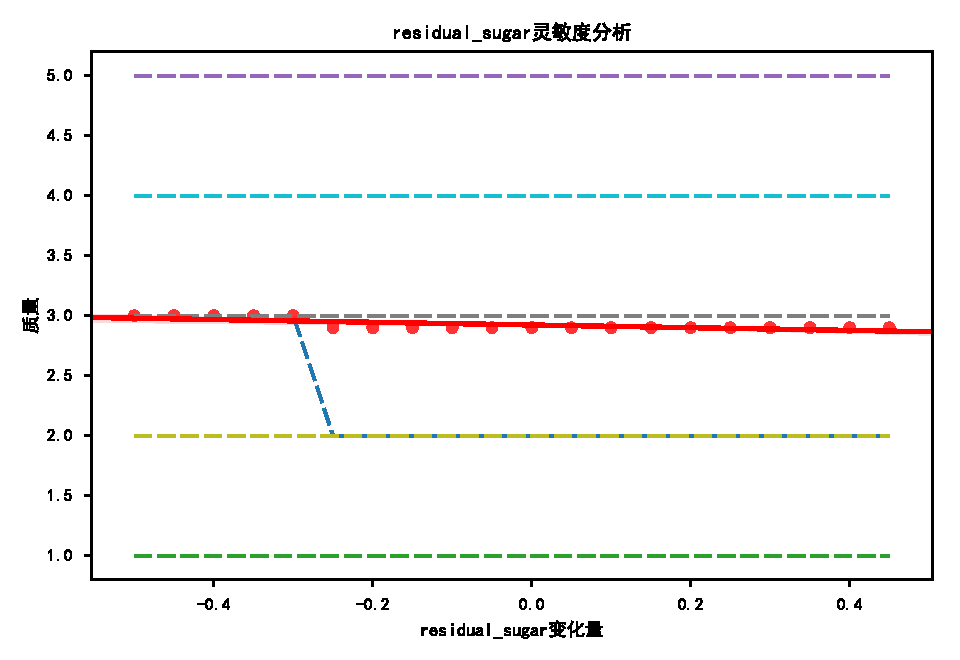
\includegraphics[width=0.99\textwidth]{sensitivity_residual_sugar.pdf}
		\caption{糖分变化对酒品质量的影响}
%		\label{fig:Anhui_trials}
	\end{minipage}
\end{figure}

\section{问题三模型的建立与求解}
\subsection{问题分析}
在前两问的基础上我们可以发现我们的模型效果还有比较大的提升空间,分析原因我们可以知道该数据的各个类别在分布上有很明显的差异,有部分等级的数据数量明显偏少,导致样本的分布不均衡,所以使得xgboost建树的过程中还是容易受到影响,所以第三问打算使用上采样方法和贝叶斯优化器的方法对该模型的数据集进行模拟扩充和参数调整,从而达到更好的效果。
\begin{figure}[!h]
	\centering
	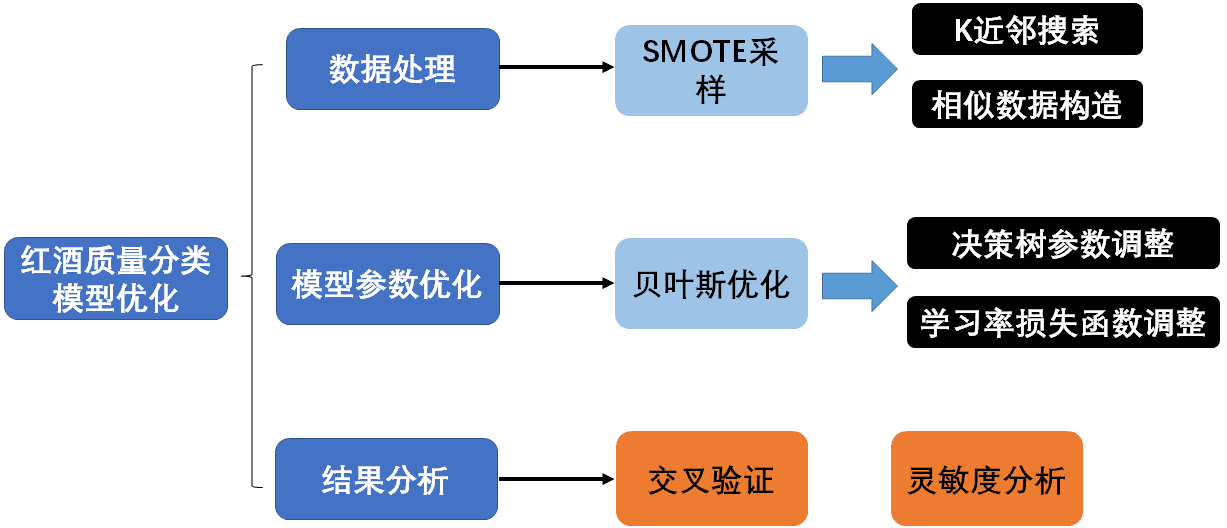
\includegraphics[width=0.7\textwidth]{map3.png}
	\caption{问题三思维导图}
\end{figure}
\subsection{上采样技术与贝叶斯优化器改进的xgboost红酒分类模型}
\subsubsection{合成少数类过采样技术}
我们通过观察发现当前数据中,质量所占样本的比例有很大的问题所以导致了预测的准确度有所下降,所以我们采用数据上采样的方法利用已知样本对数据进行构造生成相似的数据,使得当前数据的均衡度保持一致。
\begin{figure}[!h]
	\centering
	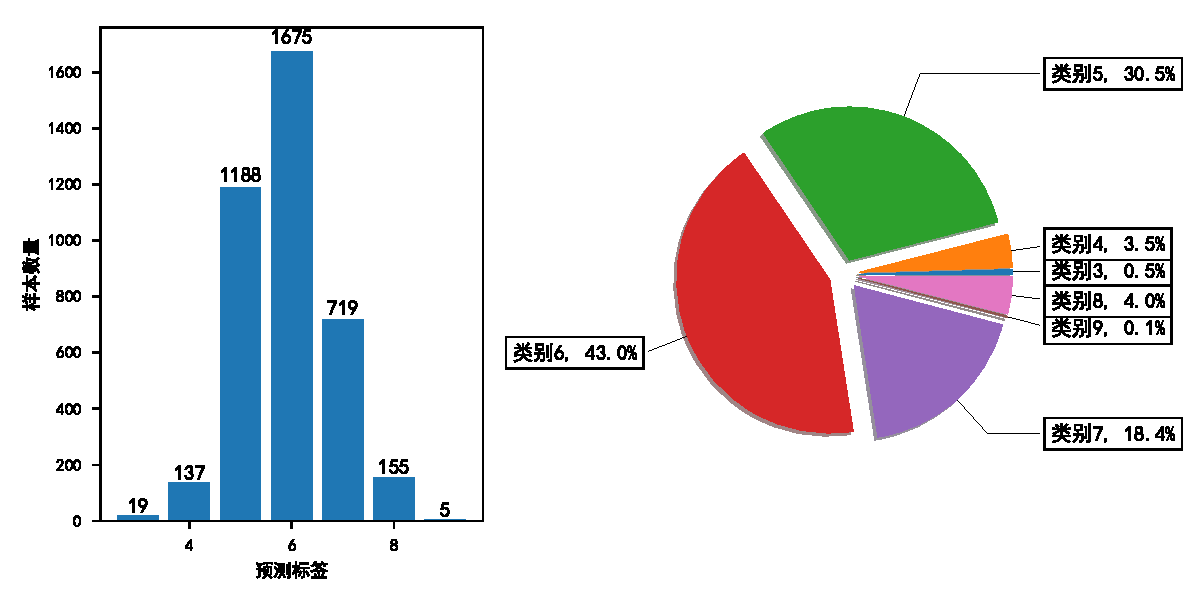
\includegraphics[width=0.7\textwidth]{labels_class_counts_data.pdf}
	\caption{原始数据质量分布不均衡现象}
\end{figure}


对于少数类中的每一个样本$x$,我们利用欧氏距离作为衡量两个样本数据差异的指标,选出它到少数类$S_{min}$中所有样本的距离得到其k近邻.
\begin{equation}
d=\sqrt{(x_{i1}-x_{j1})^2+(x_{i2}-x_{j2})^2+...+(x_{in}-x_{jn})^2}.
\end{equation}


根据样本不平衡比例设置一个采样比例以确定采样倍率n,对于每一个少数类样本x,从其k近邻中随机选择若干个样本,假设选择的近邻为xn。

对于每一个随机选出的近邻xn,分别与原样本按照公式\ref{smote}构建新的样本\upcite{bib:seven}。
\begin{equation}
x_{new}=x+rand(0,1)\times|x-xn|.
\label{smote}
\end{equation}

\begin{figure}[!h]
	\centering
	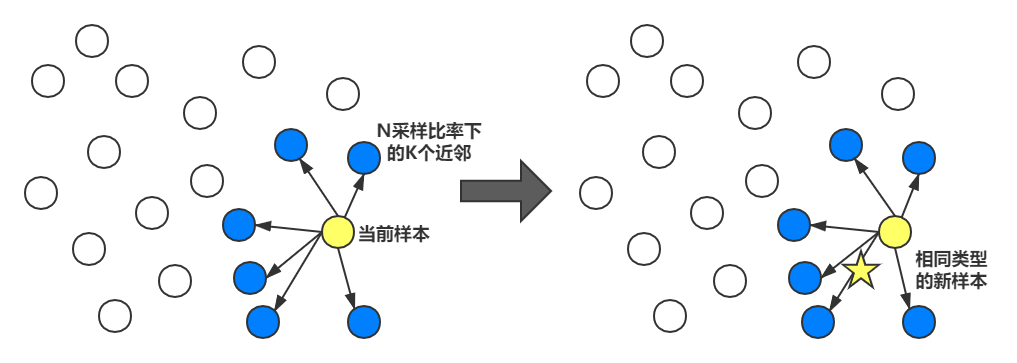
\includegraphics[width=0.8\textwidth]{caiyang.png}
	\caption{SMOTE采样原理示意图}
\end{figure}


\subsubsection{贝叶斯参数调优}
我们将微分方程所有可调节的参数设为$\mathbf{p}$,对于每一个确定的$\mathbf{p}$,我们都能求出XGBoost模型$model$.$model$输入一个数据,输出一个预测标签,即$y_i = model(x_i)$.为了对$\mathbf{p}$进行调优,我们选择针对模型在测试集上的正确率作为衡量模型好坏的标准,所以定义损失函数为模型预测错误的样本比例:
\begin{equation}
L(\mathbf{p})=1-\frac{1}{n}(\sum_{i=0}^{n-1} CORRECT_i),
\end{equation}
其中$n$为测试集样本总个数。$CORRECT_i$为一个布尔变量,表示第个样本预测正确,即:
\begin{equation}
CORRECT_i = 
\begin{cases}
1, &\text{if}\ model(i)=y_i. \\
0, & \text{if}\ model(i)\neq y_i.
\end{cases}
\end{equation}

贝叶斯优化用较少的采样数目逼近全局最优值.贝叶斯优化包含了关于$L(\mathbf{p})$的先验信念,并用从$L(\mathbf{p})$中抽取的样本更新先验,从而得到一个更好地接近$L(\mathbf{p})$的后验.用于近似目标函数的模型称为“代理模型”.贝叶斯优化还使用了一个“获取函数”,将采样导向可能优于当前最佳观测的区域.

\textbf{代理模型}(Surrogate model)
我们使用的代理模型是高斯过程Gaussian Process (GP).高斯过程是一个随机过程,其中任意点$\mathbf{x} \in \mathbb{R}^d$被赋予一个随机值$f(\mathbf{x})$,其中是这些变量的有限数量的联合高斯分布:
\begin{equation}
p(\mathbf{f} \lvert \mathbf{X}) = \mathcal{N}(\mathbf{f} \lvert \boldsymbol\mu, \mathbf{K})\label{eq1},
\end{equation}
其中$ \mathbf{f} = (f(\mathbf{x}_1),...,f(\mathbf{x}_N)), \boldsymbol\mu = (m(\mathbf{x}_1),...,m(\mathbf{x}_N)) , K_{ij} = \kappa(\mathbf{x}_i,\mathbf{x}_j)$,$m$是均值函数.高斯过程的函数的分布“平滑度”由K定义.

一个GP的先验$p(\mathbf{f} \lvert \mathbf{X})$可以在观察到一些数据$y$后转化为GP的后验$p(\mathbf{f} \lvert \mathbf{X},\mathbf{y})$,根据:
\begin{equation}
p(\mathbf{f}_* \lvert \mathbf{X}_*,\mathbf{X},\mathbf{y})= \int{p(\mathbf{f}_* \lvert \mathbf{X}_*,\mathbf{f})p(\mathbf{f} \lvert \mathbf{X},\mathbf{y})}\ d\mathbf{f}= \mathcal{N}(\mathbf{f}_* \lvert \boldsymbol{\mu}_*, \boldsymbol{\Sigma}_*).
\label{eq2}
\end{equation}

GPs定义了我们对目标函数的先验知识,我们可以使用它们来描述关于目标函数的先验信念,例如“平滑性”.GP后验计算成本低,用于在搜索空间中评估哪些采样点可能产生改进.

\textbf{获取函数}(Acquisition functions)
在搜索空间中提出采样点是通过获取函数来实现的.获取函数$u(\mathbf{x} \lvert \mathcal{D}_{1:t})$综合权衡利用(exploitation)和勘探(exploration).利用是指在替代模型预测的目标高的地方进行采样,勘探是指在预测不确定性高的地方进行采样.两者会倾向于提高采集函数值,使得获取函数最大化的采样点为下一步的试验点.
\begin{equation}
\mathbf{x}_t = \mathrm{argmax}_{\mathbf{x}} u(\mathbf{x} \lvert \mathcal{D}_{1:t-1}).
\end{equation}

\textbf{优化算法}(Optimization algorithm)
贝叶斯优化算法过程如下.

每一次参数试验执行如下步骤:

\textbf{step1.}通过代理模型(GP)求得获取函数(AF)

\textbf{step2.}通过获取函(AF)数找到下一个采样点$\mathbf{x}_t = \mathrm{argmax}_{\mathbf{x}} u(\mathbf{x} \lvert \mathcal{D}_{1:t-1})$

\textbf{step3.}对目标函数进行求值 $y_t = f(\mathbf{x}_t) + \epsilon_t$ 

\textbf{step4.}将样本$(\mathbf{x}_t,y_t)$加入先验样本 $\mathcal{D}_{1:t} = \{\mathcal{D}_{1:t-1}, (\mathbf{x}_t,y_t)\}$ 

\textbf{step5.} 更新代理模型(GP)

	

\textbf{预期提升}(Expected improvement)
定义为:
\begin{equation}
\mathrm{EI}(\mathbf{x}) = \mathbb{E}\max(f(\mathbf{x}) - f(\mathbf{x}^+), 0).
\end{equation}
其中 $f(\mathbf{x}^+)$ 是目前最优的目标函数值 $\mathbf{x}^+$ 是最优解 $\mathbf{x}^+ = \mathrm{argmax}_{\mathbf{x}_i \in \mathbf{x}_{1:t}} f(\mathbf{x}_i)$. 

预期提升可以在GP模型下求得解析解:
\begin{equation}
\mathrm{EI}(\mathbf{x}) =
\begin{cases}
(\mu(\mathbf{x}) - f(\mathbf{x}^+) - \xi)\Phi(Z) + \sigma(\mathbf{x})\phi(Z), &\text{if}\ \sigma(\mathbf{x}) > 0. \\
0,& \text{if}\ \sigma(\mathbf{x}) = 0.
\end{cases}
\end{equation}
其中:
\begin{equation}
Z =
\begin{cases}
\frac{\mu(\mathbf{x}) - f(\mathbf{x}^+) - \xi}{\sigma(\mathbf{x})}, &\text{if}\ \sigma(\mathbf{x}) > 0. \\
0, & \text{if}\ \sigma(\mathbf{x}) = 0.
\end{cases}
\label{eq:Z}
\end{equation}
式\ref{eq:Z}中的 $\xi$确定优化期间的探究量,较高的$\xi$值将导致更强的探索.$\xi$ 的推荐值是 $0.01$.


\subsection{结果分析}
该模型通过数据上采样和贝叶斯优化从而提升了当前模型的准确率,\textbf{现在该模型的准确率为}\textbf{68.4\%},\textbf{相比于第一问的结果提升}\textbf{了8.9\%}查准率与查全率相等,说明该模型已经达到了平衡点,损失函数也降低到了比较平稳的状态.


\begin{figure}[!h]
	\centering
	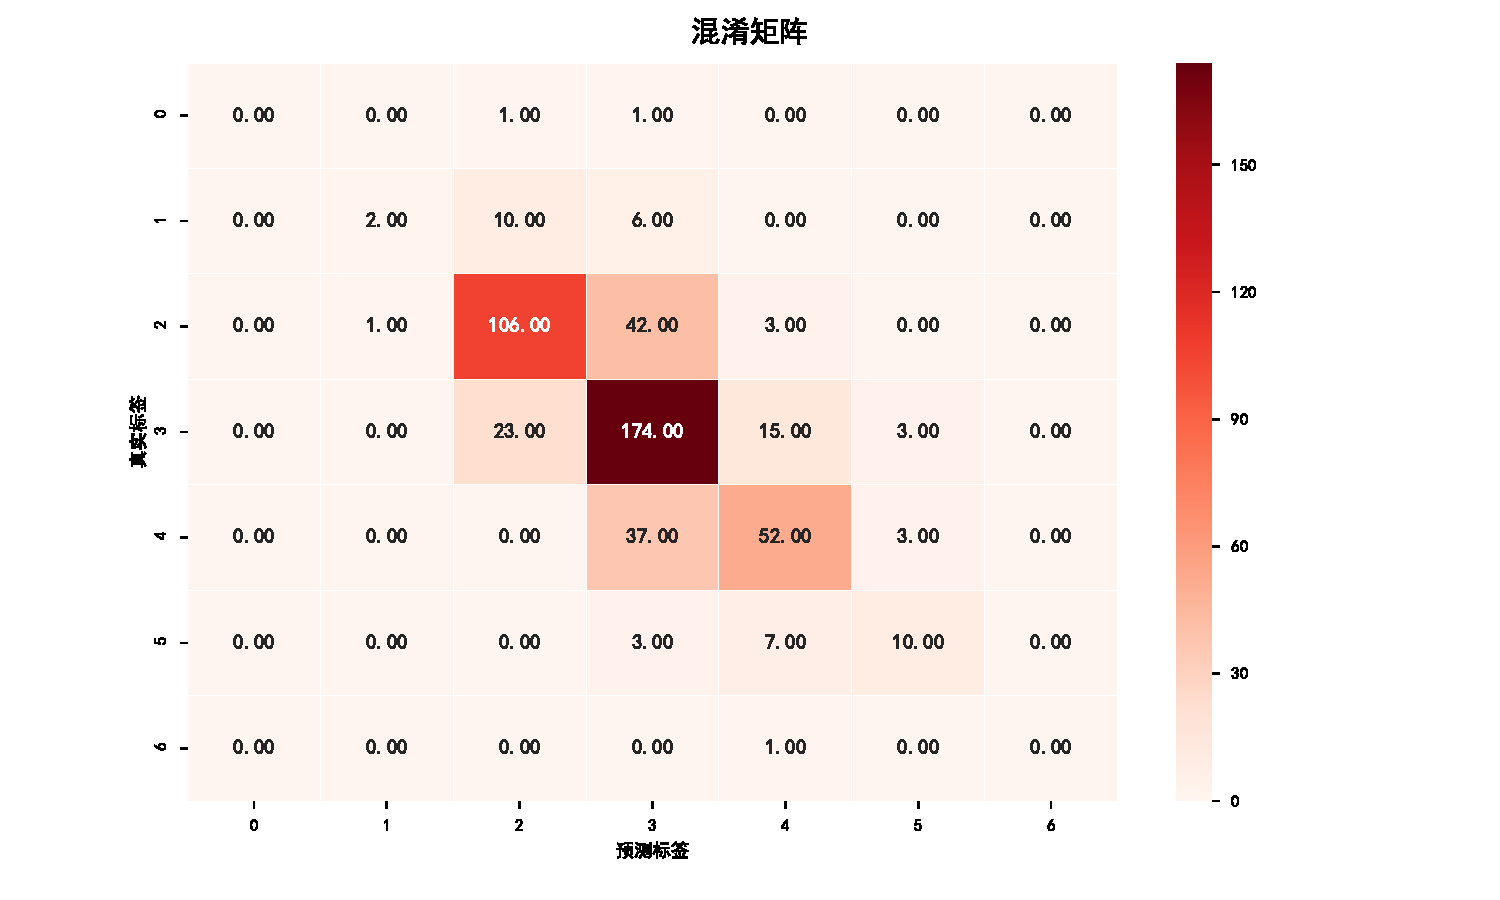
\includegraphics[width=0.8\textwidth]{cm3.pdf}
	\caption{混淆矩阵}
\end{figure}

\begin{table}[!htbp]
	\centering
	\caption{模型泛化性能}
	\begin{tabular}{crrr}
		\toprule
		& \multicolumn{1}{c}{\textbf{微平均}} & \multicolumn{1}{c}{\textbf{宏平均}} & \multicolumn{1}{c}{\textbf{加权平均}} \\
		\midrule
		\textbf{查准率precision} & 0.684 & 0.559318 & 0.687673 \\
		\textbf{查全率recall} & 0.684 & 0.438724 & 0.684 \\
		\textbf{两者的调和平均f1-score} & 0.684 & 0.472472 & 0.672773 \\
		\bottomrule
	\end{tabular}%
	\label{tab:addlabel2}%
\end{table}%

\begin{figure}[!h]
	\centering
	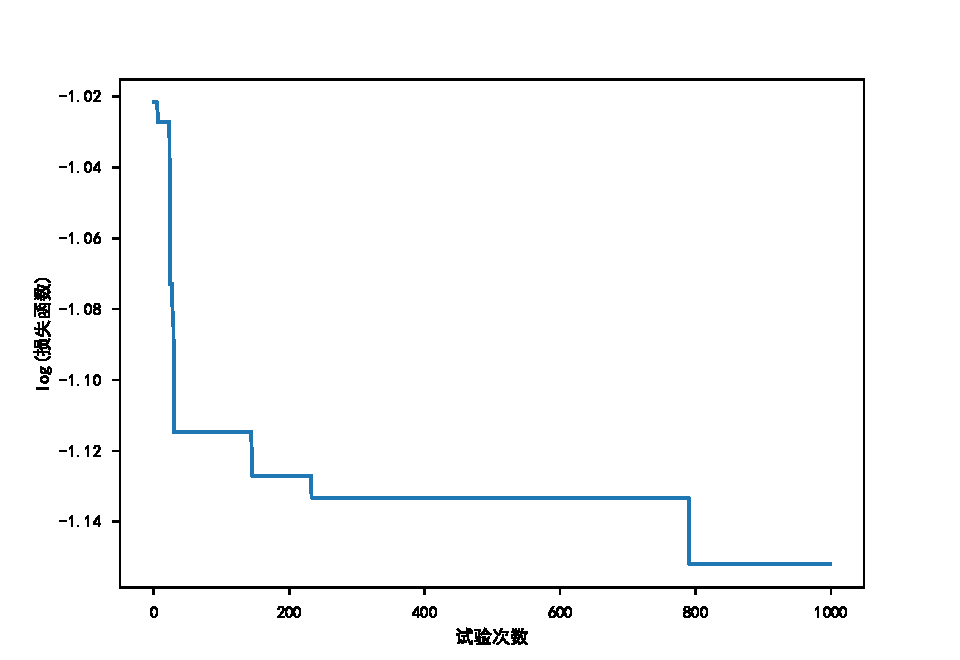
\includegraphics[width=0.6\textwidth]{_loss_time.pdf}
	\caption{损失函数}
\end{figure}

% Table generated by Excel2LaTeX from sheet 'Sheet1'



\subsection{灵敏度分析}
我们对模型的每个超参数和他的准确率进行了分析,从而确定了当前的最佳参数,从图像上我们可以看出来各个参数与准确率之间的变化趋势,\textbf{很明显当我们的树深度增加的时候,这样对于我们分类红酒的效果会更好},也能有效防止过拟合。\textbf{Gamma指定了节点分裂所需的最小损失函数下降值,这个参数的值越大,算法越保守}。这个参数的值和损失函数息息相关,分类的效果也更好,\textbf{min\_child\_weight 决定最小叶子节点样本权重和}。XGBoost的这个参数是最小样本权重的和,当它的值较大时,可以避免模型学习到局部的特殊样本。 但是如果这个值过高,会导致欠拟合,所以我们可以看到该模型中损失会随着他的增大而增大。
\begin{figure}[!h]
	\centering
	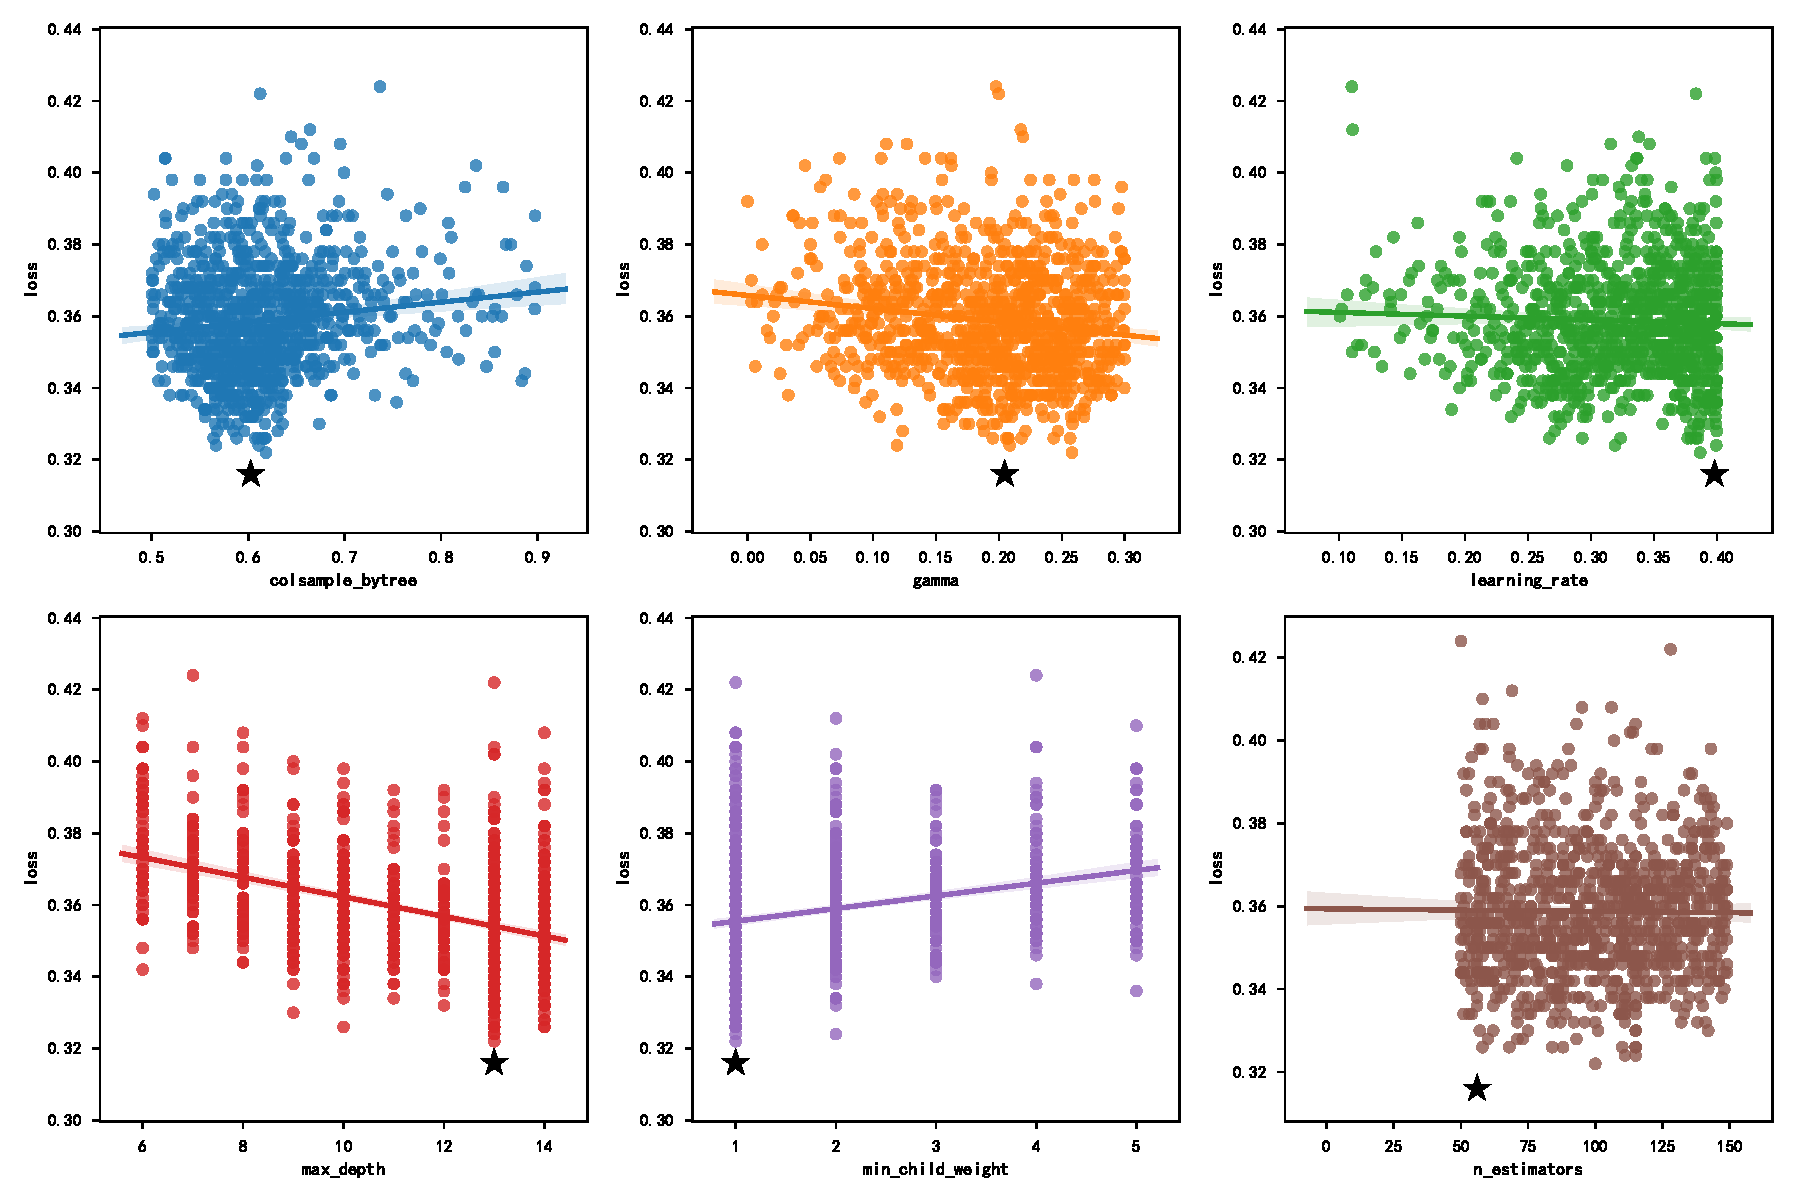
\includegraphics[width=0.8\textwidth]{_trials.pdf}
	\caption{参数对酒品质量的影响}
\end{figure}
\begin{table}[!htbp]
	\centering
	\caption{最佳参数设定}
	\begin{tabular}{cccc}
		\toprule
		\multicolumn{1}{c}{\textbf{XGBoost超参数}} & &\multicolumn{1}{c}{\textbf{XGBoost超参数}}&\\
		\midrule
		\textbf{colsample\_bytree} & 0.6026232 & \textbf{max\_depth} & 13 \\
		\textbf{gamma} & 0.2046238 &\textbf{min\_child\_weight} & 1 \\
		\textbf{learning\_rate} & 0.3980428 &\textbf{n\_estimators} & 56 \\
		\bottomrule
	\end{tabular}%
	%	\label{tab:addlabel}%
\end{table}%
\section{模型评价}

\subsection{模型的优点}
1.考虑到红酒品质预测问题必须首先进行红酒品质的分类,本文通过运用决策树与随机深林的相关理论,建立了集成决策树分类模型,使结果具有更广泛的适应性.

2.求解问题时使用xgboost算法,相较于传统GBDT算法,该算法使用二阶泰勒展开,使得求解精度跟高,同时由于进行了正则化处理,有效的控制了模型的复杂度.

3.综合三类评价指标和相关参考文献,选出了评价红酒品质的最优评价指标,理化指标影响分数的可信度较高.

\subsection{模型的缺点}
1.xgboost算法属于集成学习模型,当基分类器的个数较多时,构建模型将比较耗时。而超参数调优又需要对不同参数的模型进行大量试验,所以超参数调优将非常耗时。


\subsection{改进与展望}
对于较大的数据集,可以采用近似算法降低程序的运行时间,近似算法的核心思想是只考察分裂节点。首先根据特征分布的分位数提出候选划分点,然后将连续型特征映射到由这些候选点划分的桶中,然后聚合统计信息找到所有区间的最佳分裂点。在提出候选切分点时有两种策略,一种是学习每棵树前就提出候选切分点,并在每次分裂时都采用这种分割,第二种策略是每次分裂前将重新提出候选切分点,直观上来看,第一种策略需要更多的计算步骤,而第二种策略因为节点已有划分所以需要更多的候选点.



\appendix %%附录
%参考文献引用\upcite{bib:one,bib:two}
\begin{thebibliography}{9}%宽度9
	\bibitem{bib:one}冯嫱薇. 基于XGboost算法的信用债违约风险预测研究[D].电子科技大学,2020.
	\bibitem{bib:two}刘斌,陈凯.基于SMOTE和XGBoost的贷款风险预测方法[J].计算机与现代化,2020(02):26-30.
	\bibitem{bib:three}孙逸菲,袁德成,王建龙,白杨.基于XGBoost方法的葡萄酒品质预测[J].沈阳化工大学学报,2018,32(04):372-377.
     \bibitem{bib:four}Shutao Wang,Shiyu Liu,Jingkun Zhang,Xiange Che,Yuanyuan Yuan,Zhifang Wang,Deming Kong. A new method of diesel fuel brands identification: SMOTE oversampling combined with XGBoost ensemble learning[J].Fuel,2020,282.
     \bibitem{bib:five}李记明,姜文广.优质干红葡萄酒中主要质量指标的研究[J].中外葡萄与葡萄酒,2018(06):18-24.
     \bibitem{bib:six}司合芸. 干红葡萄酒关键工艺研究[D].江南大学,2006.
     \bibitem{bib:seven}Han H , Wang W , Mao B . Borderline-SMOTE: A New Over-Sampling Method in Imbalanced Data Sets Learning[C]. International Conference on Intelligent Computing. Springer, Berlin, Heidelberg, 2005.
%	\bibitem{bib:one} 邓纪泽. 农村饮水安全管道铺设线路设计分析[J]. 黑龙江水利科技. 2019. 47(11): 92-95.
%	\bibitem{bib:two} 于博. 浅析自来水供水管道施工技术[J]. 百科论坛电子杂志. 2019.(22): 52.
%	\bibitem{bib:three}Shiono N. Suzuki H. Saruwatari Y. A dynamic programming approach for the pipe network layout problem[J]. European journal of operational research. 2019. 277(1): 52-61.
%	\bibitem{bib:four}昝英飞. A numerical model for pipelaying on nonlinear soil stiffness seabed[J]. 水动力学研究与进展:英文版. 2016. 28(1): 10-22.
%	\bibitem{bib:five}Zhou J. Peng J. Liang G. et al. Layout optimization of tree-tree gas pipeline network[J]. Journal of Petroleum Science and Engineering. 2019. 173: 666-680.
\end{thebibliography}
\newpage
\section{代码}
\subsection{python源程序}
\lstinputlisting[language=python]{code/models.py}
\lstinputlisting[language=python]{code/paramater_tuning.py}
\lstinputlisting[language=python]{code/common.py}
\lstinputlisting[language=python]{code/read_data.py}
\lstinputlisting[language=python]{code/plot.py}
\end{document}